\section{Methodology}
\label{sec:methodology}

%Describe the methodology you have adopted, the %architecture of your system, your workflow, etc.
%Nostra metodologia: "miglioramento continuo", integrazione in base all'andamento delle metriche di prestazione. (Sommariamente, azioni? configurazione Filter, filtraggio documenti, tecniche nlp ecc.?)
%Quali metriche abbiamo preso per riferimento (presenti in treceval), strumenti e tecniche per evidenziare i problemi (es. citazione a tellme.c).
%Presenza dei diversi branch per evidenziare i flussi di lavoro paralleli per le diverse lingue.

The first goal we intended to achieve was to reach a stable and simple version of a basic indexing and searching system, to be used as a baseline to experiment additional features on. 
\par
Afterwards, the workflow split into several lines, each applying a different improvement strategy, such as different analyzing techniques, different filter configurations or different document preprocessing operations. Once a better system was found, it would eventually become the new baseline to run further experiments on.
In order to operate in this way, each line would evolve on a different working branch of our git repository, with its performance measured mainly through trec\_eval's nDCG and/or MAP metric.
\par
Some tools were also developed to help us analyze what kind of errors the run contained, to perform some pre-processing to the collection documents and to solve some translation problems.
\par
The main programming language that we used to develop our systems is Java, while some tools have been developed using Python. In particular, the core of our work was implemented by exploiting the Lucene java library~\cite{lucene}.
\par
We can split our systems in four main components:
\begin{itemize}
	\item \textbf{Parser}: it parses the corpus independently of the language chosen by using the TREC file format.
	\item \textbf{Analyzer}: it processes some text performing tokenization, stopword removal, stemming and other filtering processes.
	\item \textbf{Indexer}: it processes the parsed and analyzed documents fields to creates the index.
	\item \textbf{Searcher}: it processes a given query and exploits the index to retrieve some documents based on the processed query.
\end{itemize}

\par
In this section we describe the general workflow of our systems (Section~\ref{subsec:genflow}), the developed tools ( Sections \ref{subsec:preprocess} and \ref{subsec:transltools}), the general components (Sections \ref{subsec:parser}, \ref{subsec:analyzer}, \ref{subsec:indexer} and \ref{subsec:searcher}) and the complete systems (Section~\ref{subsec:systems}).

\subsection{General systems flow}
\label{subsec:genflow}
All of our systems operate in the following order (a scheme of the system is reported in Figure~\ref{fig:overallsys}):
\begin{enumerate}
	\item Apply a pre-processing to the documents of the corpus (optional stage).
	\item Parse the documents of the corpus, splitting the content into the appropriate fields, using the parser.
	\item Analyze the documents' fields to convert them into a stream of tokens and index them to perform the search (single index folder).
	\item Parse and analyze the queries to convert them into a stream of tokens.
	\item Perform the search by exploiting the index (one query at the time).
	\item Rerank the documents retrieved with the search (optional stage).
	\item Print the results of the search into a dedicated text file.
\end{enumerate}

\begin{figure}[tb]
    \centering
    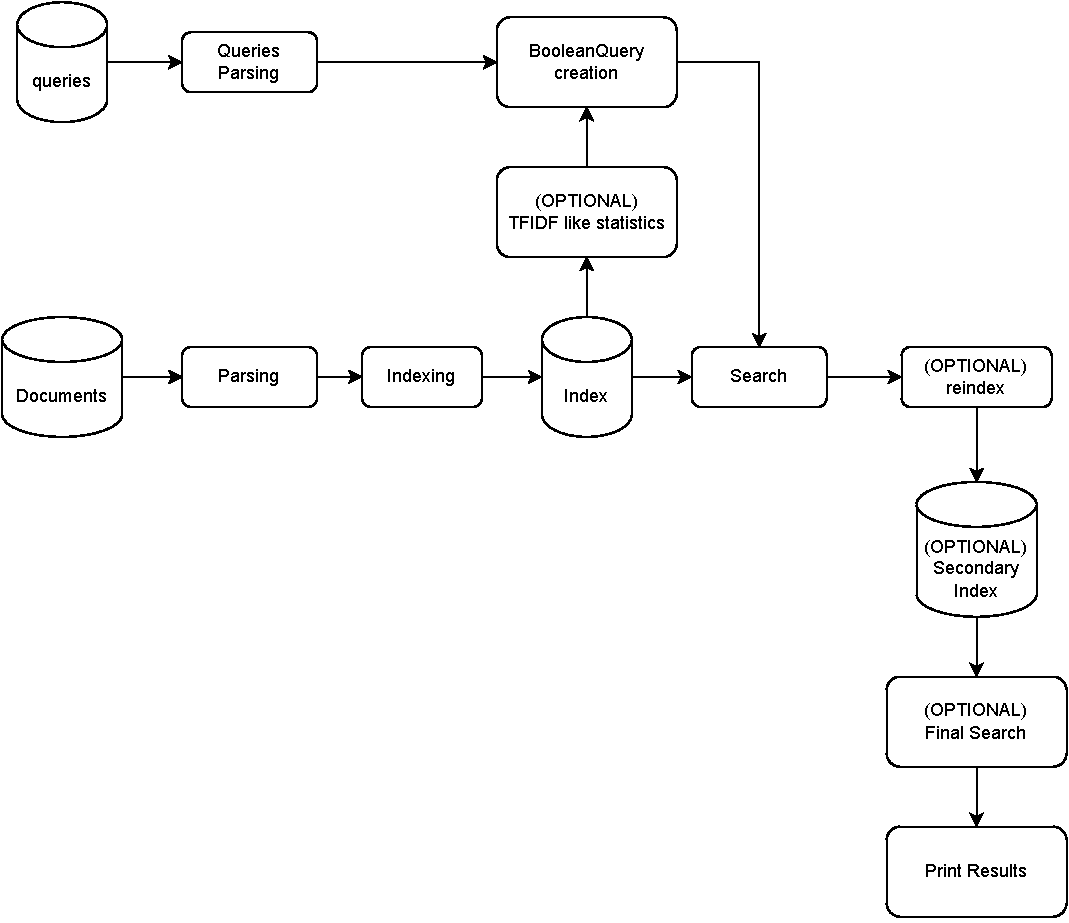
\includegraphics[scale=0.8]{figure/overallsystem.pdf}
    \caption{General system scheme}
    \label{fig:overallsys}
\end{figure}

\subsection{Pre-processing tools}
\label{subsec:preprocess}
\subsubsection{SPAM parser}
\label{subsubsec:spam}
By analyzing the results produced with the French-based system (the simplest one) on the French collection, we realized that relevant documents for a specific query were not included in the first one thousand documents retrieved by the system for that query. Before increasing the system's complexity through new features, while inspecting the retrieved documents, it turned out that several of the non-relevant documents were actually ranked as relevant documents due to the high number of words repetitions inside them. More precisely, excluding documents that were actually not relevant, we noticed that in the analyzed documents the words were not different and the text contained a sensible number of repetitions. This new information drove us to develop term frequency analyses to avoid the retrieval of documents considered "spam" during the search task or, even better, the addition to the Lucene index during the index task, reducing its overall size.  
\par
With the term "spam" we denote the type of documents that "hack" the retrieval system through the use of a set of words contained in the user query, that brings the document to the top of the document-ranked list.   
\par
The following documents are some examples of "spam". We can notice that the length of the texts is very short compared to the one of an average document: 
\begin{quote}
    \centering \textit{"\textbf{Tableau} de conversion pouce / inch en Cm mm | \textbf{Tableau} de conversion, \textbf{Tableau} de conversion de mesure, Scrapbooking à imprimer"} 
\end{quote}
\begin{quote}
    \centering  \textit{"[...] \textbf{Quiz} : Cinéma \textbf{Quiz} : Histoire de France \textbf{Quiz} : Géographie \textbf{Quiz} : Histoire \textbf{Quiz} : Littérature \textbf{Quiz} : Espace \textbf{Quiz} : Bien-être \textbf{Quiz} : Littérature \textbf{Quiz} : Gamer \textbf{Quiz} : Formule 1 \textbf{Quiz}"[...] }
\end{quote}
The methodology that we applied to fulfil this goal takes into account two main factors:  
\begin{enumerate}
    \item The ratio between the most frequent word and the total length of the document, excluding articles and stopwords: 
    \begin{equation}
        \frac{\text{Max freq}}{\text{Doc length}}.
    \end{equation} 
    The value obtained is as low as the term occurrences are spread all over the document.
    \item The ratio between the number of words in the document and the number of different words used in it:
    \begin{equation}
        \frac{\text{Doc length}}{\text{Number different words}}.
    \end{equation} This value reaches higher values for documents which contain the same few words repeated many times. For this reason, they may not contain any useful information for the user.  
\end{enumerate}
In order to combine the two approaches, we can obtain a third ratio by multiplicating the previous ones and comparing the result with a threshold:
\begin{equation}
    \frac{\text{Max freq}}{\cancel{\text{Doc length}}} \cdot \frac{\cancel{\text{Doc length}}}{\text{Number different words}} = \frac{\text{Max freq}}{\text{Number different words}} > \text{threshold}
\end{equation}
\par
During the process, one more threshold is checked: the length of the analyzed word. Since the implemented parser splits the sentences using blank spaces, it may happen that sequence of characters (e.g. "$\star \star \star$", "NVO",..) or symbols (e.g. €) cause an erroneous document exclusion. By applying the proposed threshold these errors are avoided. 
\par
The entire pre-processing task was implemented in a separate Python file which automatically reads all the files in the French collection and for each file it saves a new one that doesn't contain the documents marked as spam. The overall flow is reported in Figure\ref{fig:doc_parser-figure}. 

\begin{figure}[tb]
  \centering
  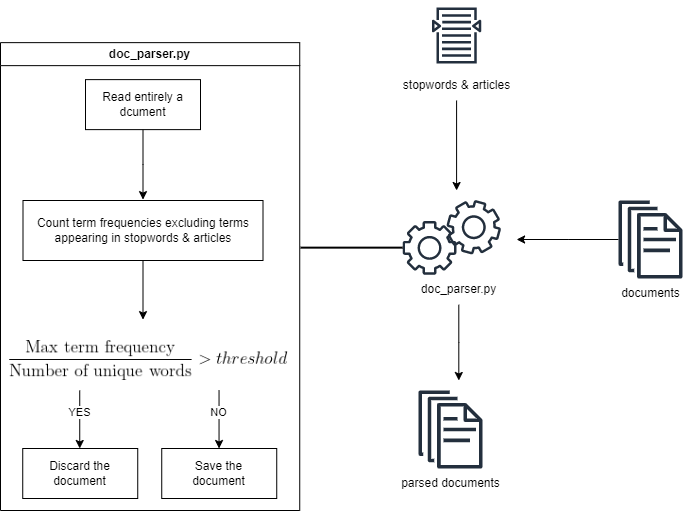
\includegraphics[width=250px,scale=0.5]{figure/doc_parser-diagram.png}
  \caption{Flow of the documents parser. (\href{https://bitbucket.org/upd-dei-stud-prj/seupd2223-dards/src/french/docs_filter.py}{docs\_filter.py}).}
  \label{fig:doc_parser-figure}
\end{figure}

\subsubsection{Synonyms}
\label{subsubsection:synonyms}
In order to try to increase the system's performance, a query expansion method was implemented through the use of synonyms. The files containing French synonyms available on the internet were not sufficient and covered only a small part of the entire French dictionary. For this reason, a new collection of words that could be easily used as synonyms of words found in the queries during the search task was needed. To address this need, another Python tool that automatically performs a request to a specialized site \url(dictionary.reverso.net/french-synonyms/) and retrieves all the related synonyms was created. All the new words found are placed in the same line as the searched word so that the Searcher (\ref{subsec:searcher}) can easily extract the information needed. The overall flow is shown in Figure~\ref{fig:search_synonyms-figure}.

\begin{figure}[tb]
  \centering
  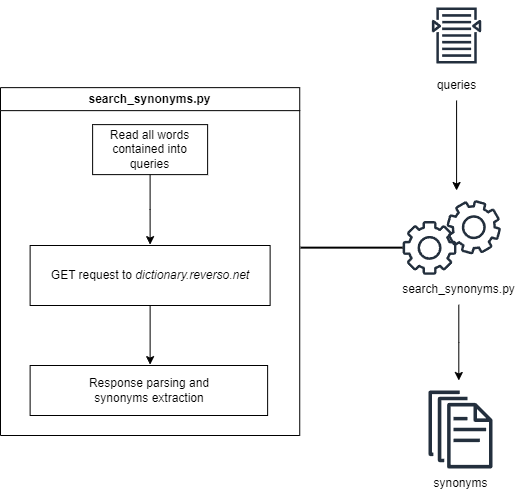
\includegraphics[width=250px,scale=0.5]{figure/search_synonyms.png}
  \caption{Flow of the synonyms searcher. (\href{https://bitbucket.org/upd-dei-stud-prj/seupd2223-dards/src/french/search_synonyms.py}{search\_synonyms.py}).}
  \centering \label{fig:search_synonyms-figure}
\end{figure}


\subsection{Translation tool}
\label{subsec:transltools}
Since the translations of the documents and the queries provided by CLEF resulted to be imprecise, we developed a tool that allows to translate a piece of text from French to English.
The tool has been implemented as a script in Google's "Google App Script" platform and then deployed as a web application. This tool must be used as a REST resource.
\par
The code used to implement this tool can be found \href{https://bitbucket.org/upd-dei-stud-prj/seupd2223-dards/src/master/code/BM25TRANSLATEDQUERIES/src/main/java/it/unipd/dei/dards/utils/GoogleScriptApi.gs}{HERE}.


\subsection{Parser}
\label{subsec:parser}
The parser that we implemented for all of our systems is a basic parser. This component simply reads all the files with a given extension (.txt) present in a directory tree (specified as input) and converts all the \textbf{Trec} formatted documents into an instance of document that has two fields: the identifier of the document (ID) and the body of the document (BODY). Some systems in addition to that also read another file (whose path is given as input) that contains pairs "document identifier"-"document url" and add an additional url field (URL) to the instances of the documents based on the identifier. In some systems, we decided to add this field for two reasons: the URL could help decreasing the rank position of the document containing "spam" (see section~\ref{subsec:preprocess}) and it could help us in the queries that contain a website url.
\par
Furthermore, we tried also to add another field to the document instances that was meant to contain the document keywords (retrieved exploiting an algorithm called RAKE~\cite{rake}, Rapid Automatic Keyword Extraction), but it required too much computation time so we didn't implement this option.
\par
Eventually, the parsing of the queries uses the \textbf{tsv} file format and it is done in the searcher module (see Section~\ref{subsec:searcher}).


\subsection{Analyzer}
\label{subsec:analyzer}
In our systems we implemented customized analyzers instead of using the standard ones proposed by Lucene. This choice was motivated by the fact that this way we could customize the filters pipeline and choose a tokenizer. Tokenizers process the input stream (the document text) and using some predefined rules they split it into tokens: these are the atomic units composing a document. Unlike words, tokens do not have to be grammatically correct or meaningful, but are suitable for processing and comparison operations.
We tried two different tokenizers:
\begin{itemize}
    \item \textbf{StandardTokenizer}: a grammar-based tokenizer constructed with JFlex. It implements the Word Break rules from the Unicode Text Segmentation algorithm, as specified in Unicode Standard Annex \#29.
    \item \textbf{WhiteSpaceTokenizer}: it breaks text into terms whenever it encounters a whitespace character.
\end{itemize}
We started out using StandardTokenizer and we noticed that expressions separated with hyphens were divided into different tokens. To avoid this, we tried a combination of WhiteSpaceTokenizer and PatternReplaceFilter to remove all punctuations/symbols except for hyphens. But then performance decreased and we backtracked.
\\
In addition to the StandardTokenizer we used different filters, some of them shared by both English-based and French-based systems:
\\
\textbf{French}
\begin{itemize}
    \item \textbf{ElisionFilter}: it targets elisions, so removes articles, prepositions and conjunctions placed either in the initial or final part of the token, usually connected by an apostrophe or hyphen. This connection makes it impossible for a generic stopword filter alone to detect and delete those particles.
    \item \textbf{ASCIIFoldingFilter}: it converts alphabetic, numeric, and symbolic Unicode characters which are not in the Basic Latin Unicode block (the first 127 ASCII characters) to their ASCII equivalents, if one exists. This filter was used to solve accents and diacritical marks problem with French.
    \item \textbf{FrenchLightStemFilter}: this stemmer implements the "UniNE" algorithm~\cite{frenchlightstemmer}.
\end{itemize}
Note that for the French case other stemmers (FrenchMinimalStemmer, org.taurus.snowball's FrenchStemmer) and chain of stemmers (multiple stemmers in a single analyzer) have been tested and evaluated but the performance of the FrenchLigthStemmer turned out to be the best.
\\
\textbf{English}
\begin{itemize}
    \item \textbf{NGramFilter}: it generates character n-gram tokens of sizes in the given range. Tokens are ordered by position and then by gram size.
    \item \textbf{ShingleFilter}: it constructs word n-grams, which are token n-grams, from the token stream.
    \item \textbf{PorterStemFilter}: it applies the Porter Stemming Algorithm for English. The results are similar to using the Snowball Porter Stemmer with the language="English" argument. It is coded directly in Java and it is four times faster than the English Snowball stemmer.
    \item \textbf{KStemFilter}: it is an alternative to the Porter Stem Filter for developers looking for a less aggressive stemmer. KStem was written by Bob Krovetz, ported to Lucene by Sergio Guzman-Lara (UMASS Amherst). This stemmer is only appropriate for English language text.
\end{itemize}

\textbf{Shared}
\begin{itemize}
    \item \textbf{LowerCaseFilter}: it converts any uppercase letter in a token to the equivalent lowercase token. All other characters are left unchanged.
    \item \textbf{StopFilter}: it discards, or stops analysis of, tokens that are on the given stop words list.
    \item \textbf{SynonymGraphFilter}: it maps single- or multi-token synonyms, producing a fully correct graph output. If used for indexing it must be followed by a FlattenGraphFilter to squash tokens on top of one another, because the indexer can’t directly consume a graph.
    \item \textbf{HyphenatedWordsFilter}: it reconstructs hyphenated words that have been tokenized as two tokens because of a line break or other intervening whitespace in the field test. If a token ends with a hyphen, it is joined with the following token and the hyphen is discarded.
    \item \textbf{RemoveDuplicatesTokenFilter}: it removes duplicate tokens in the stream. It filters out Tokens at the same position and Term text as the previous token in the stream.

    \item \textbf{NumberFilter}: it removes every token in the token stream that happens to be a number (this filter has been developed by team DARDS).
\end{itemize}


\subsection{Indexer}
\label{subsec:indexer}
The indexer's job is to store the tokens, generated by processing every document with a given analyzer, into an inverted index (data structure which maps terms to documents).
We implemented two types of indexer, \textit{DirectoryIndexer} and \textit{ReRankDirectoryIndexer}, the first one takes all the documents in a given directory and stores them into the index, the second one does the same but it can also store a list of documents passed to it.
\\
Lucene captures some statistics at indexing time which can then be used to support scoring at query time. To do this it makes use of similarity functions, which set a per-document value for every field in the document. Hence, the similarity determines how Lucene weights terms.
\\
In our systems we tested different similarities:

\begin{itemize}
    \item \textbf{BM25Similarity}: it implements the Okapi BM25 (Best Match, attempt 25).
    \item \textbf{LMDirichletSimilarity}: bayesian smoothing using Dirichlet priors. The formula assigns a negative score to documents that contain the term, but with fewer occurrences than predicted by the collection language model.
    \item \textbf{LMJelinekMercerSimilarity}: language model based on the Jelinek-Mercer smoothing method. The model has a single parameter, $\lambda$. The optimal value is around 0.1 for title queries and 0.7 for long queries. Values near zero act score more like a conjunction (coordinate level matching), whereas values near 1 behave the opposite (more like pure disjunction).
    \item \textbf{DFRSimilarity}: it implements the divergence from randomness (DFR) framework. Probabilistic models of IR based on measuring the divergence from randomness. The DFR scoring formula is composed of three separate components: the basic model, the aftereffect and an additional normalization component.
    \item \textbf{ClassicSimilarity}: subclass of TFIDFSimilarity. Lucene combines Boolean model (BM) of Information Retrieval with Vector Space Model (VSM) of Information Retrieval. In VSM, documents and queries are represented as weighted vectors in a multi-dimensional space, where each distinct index term is a dimension, and weights are Tf-idf values. VSM score of document d for query q is the Cosine Similarity of the weighted query vectors V(q) and V(d).
    \item \textbf{BooleanSimilarity}: it gives terms a score that is equal to their query boost.
    \item \textbf{AxiomaticF2LOG}: it is defined as $ \sum tfln(\textup{term\_doc\_freq}, \textup{docLen}) \times \textup{IDF(term)}$ whit $\textup{IDF(term)}=ln \left(\frac{N+1}{df(t)}\right)$; where $N$ equals total number of docs, $df$ corresponds to the docs frequency.
    \item \textbf{AxiomaticF2EXP}: it is defined as $ \sum tfln(\textup{term\_doc\_freq}, \textup{docLen}) \times \textup{IDF(term)}$ whit $\textup{IDF(term)}= \left({\frac{N+1}{df(t)}}\right)^k$; where $N$ equals total number of docs, $df$ corresponds to the docs frequency.
    \item \textbf{IndriDirichletSimilarity}: bayesian smoothing using Dirichlet priors as implemented in the Indri Search engine. A larger value for parameter $\mu$ produces more smoothing. Smoothing is most important for short documents where the probabilities are more granular.
    \item \textbf{MultiSimilarity}: particular similarity which implements CombSUM method for combining evidence from multiple similarity values~\cite{multisim}.
\end{itemize}
In the large majority of cases the BM25Similarity turned out to be the best option to use (see Table~\ref{tab:similcomp}. Note that the values of the following table refer to an initial system that performed the search on the English corpus provided by CLEF).
\begin{center}
\begin{table}[tb]
\centering
\begin{tabular}{|l|c|} 
 \hline
    \textbf{Similarity} &  \textbf{MAP}  \\
 \hline\hline
 BM25Similarity & 0.1424  \\ 
 LMJelinekMercerSimilarity(0.1F) & 0.1249   \\
 LMJelinekMercerSimilarity(0.5F) & 0.1255  \\
 LMJelinekMercerSimilarity(0.8F) & 0.1242  \\ 
 DFRSimilarity (most of the configurations)& 0.1423\\
 LMDirichletSimilarity & 0.1204\\
 IndriDirichletSimilarity & 0.0137 \\
 ClassicSimilarity & 0.0740\\
 BooleanSimilarity & 0.0121 \\
 AxiomaticF2LOG & 0.1358 \\
 AxiomaticF2EXP & 0.1346\\
 \hline
\end{tabular}
\caption{Comparison of rerank performance.}
\label{tab:similcomp}
\end{table}
\end{center}

\subsection{Searcher}
\label{subsec:searcher}
The searcher is the other fundamental part of any IR system besides the Indexer. This component takes care of doing the matching between a document and a topic, giving as a result a ranking, which marks how relevant a document should be for a certain topic. In our application, topics are real user queries.
\par
In our systems, the searcher have been customized to first parse the queries from a provided, .tsv formatted file. Then, one query at the time, this component turns the query into a stream of tokens (exploiting a query parser and an analyzer which must be the same used for indexing), converts it into a Lucene Query and searches the index for it. After performing the actual search this tool optionally executes a rerank (see Section~\ref{subsub:rerank}) and then prints the results of the overall process into a file.
\par
Note that in some systems the query is not directly turned into a Lucene Query but in the process the terms are boosted (see Section~\ref{subsub:boost}). Furthermore, in the majority of cases the query is performed by considering the BODY field of the document but in some systems the same query is applied also to the URL field.

\subsubsection{Boosting}
\label{subsub:boost}
In some of our systems we decided to not to use a plain query but to boost the term according to some statistics. In particular, we computed a boost factor based on a measure that is quite similar to the the TF-IDF weight. The equations used to compute the boost factor for the term \textit{i} are the following:
\begin{equation}
 w_i={\left(\frac{ttf_i}{\sum_{j} ttf_j}\right)}^{0.2} \cdot \left(1+\log \frac{N+1}{n_i+1} \right),
\end{equation}
where with $ttf_i$ we indicate the "total term frequency" (number of occurrences of the term in the entire corpus), with $N$ the number of documents in the corpus and with $n_i$ we denote the number of documents containing the term.

\par
In order to boost the query terms we:
\begin{enumerate}
    \item Compute from the index an hash map that contains as keys the terms and as values the related weight.
    \item Get (exploiting the analyzer), from the original text of the query, the list of terms that will compose our Lucene Query.
    \item Create a TermQuery for each of the term.
    \item Wrap the TermQuery in a BoostQuery, setting the boost based on the hash map (the boost is set to zero if the term doesn't appear in the index).
    \item Merge all the BoostQuery(ies) in a BooleanQuery.
\end{enumerate}


\subsubsection{Reranking}
\label{subsub:rerank}
%Descrizione in breve: cos'è, cosa fa, a cosa serve. Effetto in generale (risultati descritti su sistema relativo).
After the searcher performed the task, some systems execute a rerank. To implement the reranking we simply consider the document retrieved by the search (hits), we create a new index based only on those documents (or only on the top-N document retrieved) and eventually we repeat the same or a slightly modified query (depending on the system) on the new index.


\subsection{Systems}
\label{subsec:systems}
In this subsection we describe the systems that we implemented. The overall system sequence diagram is reported in Figure~\ref{fig:overallsys}.



\subsubsection{BM25FRENCHBASE system}
\label{subsub:BM25FRENCHBASE}
As a baseline for all our work, this IR system for French uses:
\begin{table}[h!]
    \centering
    \begin{tabular}{l p{0.8\linewidth}}
    Query language & French\\
    Document language & French\\
    Preprocessing & None\\
    Similarity & BM25Similarity\\
    Analyzer & Custom, composed as below\\
    Tokenizer & StandardTokenizer\\
    Filters & ElisionFilter, LowerCaseFilter, StopFilter, ASCIIFoldingFilter, FrenchLightStemFilter\\
    Searcher & Standard searcher
    \end{tabular}
\end{table}
\par This configuration has been achieved by trying all possible filter configurations while retaining only the better performing ones.
\\
The stoplist used by the StopFilter is a custom stoplist created by merging different French stoplist found online and by adding some terms based on the index created (that has been analyzed using Luke).
\\ 
The article's list used by the ElisionFilter is a custom list of terms that we created on the basis of French dictionaries. 
\\
The ASCIIFoldingFilter was used to avoid problems related to French diacritical marks and accents since not in all queries and/or documents were used properly.
\par
This system has overall good performance on the test data, especially considering its moderate complexity.

\subsubsection{BM25FRENCHBOOSTURL system}
\label{subsub:BM25FRENCHBOOSTURL}
The BM25FRENCHBOOSTURL system considers a document with three fields: ID,BODY,URL (see Section~\ref{subsec:parser}). Furthermore this system uses:
\begin{table}[h!]
    \centering
    \begin{tabular}{l p{0.8\linewidth}}
    Query language & French\\
    Document language & French\\
    Preprocessing & None\\
    Similarity & BM25Similarity\\
    Analyzer & Custom, composed as below\\
    Tokenizer & StandardTokenizer\\
    Filters & ElisionFilter, LowerCaseFilter, StopFilter, ASCIIFoldingFilter, FrenchLightStemFilter\\
    Searcher & Standard searcher + boosting (see Section~\ref{subsub:boost})
    \end{tabular}
\end{table}
\\
In this system the query is performed on both the BODY field and the URL field of the document but in a slightly different way. In particular, the main boolean query is composed of two sub-queries: one for the BODY field where each term is connected by means of an OR clause, the other for the URL field where term is connected by means of an AND clause. Eventually, the two sub-queries are connected by means of an OR clause to compose the final query.
\par
Furthermore, boosting is performed, as described in Section~\ref{subsub:boost}, in the same way for both the URL and BODY field sub-queries (we tried different combination of boosting, for example to give to the URL sub-query terms double the weight, but this combination turned out to be the best).
\par
The stoplist used by the StopFilter is a custom stoplist created by merging different French stoplist found online and by adding some terms based on the index created (that has been analyzed using Luke).
\par 
The article's list used by the ElisionFilter is a custom list of terms that we created on the basis of French dictionaries. 
\par
The ASCIIFoldingFilter was used to avoid problems related to French diacritical marks and accents since not in all queries and/or documents were used properly.

\subsubsection{BM25TRANSLATEDQUERIES system}
\label{subsub:BM25TRANSLATEDQUERIES}
The BM25TRANSLATEDQUERIES system has been developed as an attempt of running an English system with a better query quality: looking at the supplied English queries, multiple translation mistakes and imprecisions were noticeable (see Table~\ref{tab:qtransl} for some examples).
\begin{table}[tb]
  \caption{Query translation error examples}
  \label{tab:qtransl}
  \centering
  \begin{tabular}{|l|l|p{0.6\linewidth}|}
    \toprule
    Query ID&French&English\\
    \midrule
    q062213307 & cuisson gigot agneau & leg leg leg leg leg leg leg leg leg leg leg leg leg leg leg leg leg leg leg leg leg leg leg leg leg leg leg leg leg leg leg leg leg leg leg leg leg leg leg leg leg leg leg leg leg leg leg leg leg leg leg leg leg leg leg leg leg leg leg leg leg leg leg leg leg leg leg leg leg leg leg leg leg leg leg leg leg leg leg leg leg leg leg leg leg leg leg leg leg leg leg leg leg leg leg leg leg leg leg leg leg leg leg leg leg leg leg leg\\
q062228 & aeroport bordeaux & airport\\
  \bottomrule
\end{tabular}
\end{table}
Therefore, a custom translator was implemented, as defined in Section~\ref{subsec:transltools}.
\par
The translation of the queries is performed in the searcher right after their parsing and before turning them into a token stream.
\par
This system uses:
\begin{table}[h!]
    \centering
    \begin{tabular}{l p{0.8\linewidth}}
    Query language & French, translated in English\\
    Document language & English\\
    Preprocessing & None\\
    Similarity & BM25Similarity\\
    Analyzer & Custom, composed as below\\
    Tokenizer & StandardTokenizer\\
    Filters & LowerCaseFilter, StopFilter, KStemFilter\\
    Searcher & Standard searcher + query translation
    \end{tabular}
\end{table}
\\
By doing several experiments we noticed that with English the best performing stemmer was the Krovetz stemmer (\textit{KStemFilter}).
\par
The StopFilter does not use a customized stoplist but it uses the standard English stoplist provided by the Lucene class EnglishAnalyzer through the static variable ENGLISH\_STOP\_WORDS\_SET.
\par
Furthermore, to increase the performance, we tried to translate also the documents by using our tool (see Section~\ref{subsec:transltools}) but, since the tool is used as a REST resource and because of the number and length of the documents, this approach resulted to be too demanding in terms of computational time, so we abandoned this idea.

\subsubsection{BM25FRENCHRERANK100 system}
\label{subsub:BM25FRENCHRERANK100}
%Questo sistema implementa reranking + boost MA senza boost x campo URL.
This system has been developed to evaluate the benefits of introducing reranking mechanics (as defined in Section~\ref{subsub:rerank}).
In order to achieve a better performance, query boosting (see Section~\ref{subsub:boost}) is also included in the Searcher. In comparison to  \ref{subsub:BM25FRENCHBOOSTURL}, this system does not take into account the document's URL but it considers only the BODY and ID fields.
\par Here follows a more detailed component overview:
\begin{table}[h!]
    \centering
    \begin{tabular}{l p{0.8\linewidth}}
    Query language & French\\
    Document language & French\\
    Preprocessing & None\\
    Similarity & BM25Similarity\\
    Analyzer & Custom, composed as below\\
    Tokenizer & StandardTokenizer\\
    Filters & ElisionFilter, LowerCaseFilter, StopFilter, ASCIIFoldingFilter, FrenchLightStemFilter\\
    Searcher & Standard searcher + boosting (see Section~\ref{subsub:boost}) + reranking
    \end{tabular}
\end{table}
\par
The rerank is performed as described in Section~\ref{subsub:rerank} and, in this case, the query that is used to repeat the search is the same used for the main search. The query created is a BooleanQuery obtained by connecting the BoostedQuery(ies) (each representing a boosted token of the topic ) by means of an OR clause.
\par
Note that this system performs the rerank only for the first (most relevant) 100 document retrieved by the first search (for the CLEF LongEval task the maximum number of retrieved documents is 1000). We have chosen to rerank only 100 documents because by looking at the performance through the Trec\_Eval tool we noticed that the recall at the document cut-off 100 was sufficiently high. Nonetheless, we also tried to perform the rerank considering all the retrieved document but the performance resulted to be lower. 
\par
Finally, we tried to boost the query performed in the second search in a different way (by recomputing the TF-IDF-like weights considering only the secondary index created in during the reranking step) but the performance decreased (see Table~\ref{tab:rerankperf}).

\begin{center}
\begin{table}[tb]
\centering
\begin{tabular}{|l|c|c|} 
 \hline
   & rerank100 & rerank1000  \\
 \hline\hline
 MAP & 0.1960 & 0.1702 \\ 
 nDCG & 0.3657 & 0.3379  \\
 recall & 0.8437 & 0.8437 \\
 p@5 & 0.1533 & 0.1336 \\ 
 \hline
\end{tabular}
\caption{Comparison of rerank performance.}
\label{tab:rerankperf}
\end{table}
\end{center}
\par
The stoplist used by the StopFilter is a custom stoplist created by merging different French stoplist found online and by adding some terms based on the index created (that has been analyzed using Luke).\\
The article’s list used by the ElisionFilter is a custom list of terms that we created on the basis of French dictionaries.\\
The ASCIIFoldingFilter was used to avoid problems related to French diacritical marks and accents since not in all queries and/or documents were used properly.

\subsubsection{BM25FRENCHSPAM system}
\label{subsub:BM25FRENCHSPAM}
The system BM25FRENCHSPAM implements entirely the BM25FRENCHBASE (\ref{subsub:BM25FRENCHBASE}) applying documents preprocessing. All documents used as input are first parsed by a "spam" parser implemented in Python, as described in Section~\ref{subsubsec:spam}, and executed before the BM25FRENCHSPAM analyses. Since the pre-process activity uses a threshold above which a document is excluded, it was necessary to understand the average value (\(\frac{\text{Max freq}}{\text{Number different words}}\)) of the collection, assuming that most of the documents were valid (i.e. contain meaningful sentences). Using a slightly modified version (not reported) of the already existing parser (Figure~\ref{fig:doc_parser-figure}) it turned out that the average ratio of the test collection corresponded to 6.5\%. 
\par
In order to assign as correct a value as possible, some test has been done using different thresholds and checking the corresponding performance.  More specifically, the considered tested values are 7\%, 9\%, 11\% and 15\% and the performance are reported in Table~\ref{tab:spamparsingperf}.
\begin{center}
\begin{table}[tb]
\centering
\begin{tabular}{|l|c|c|c|c|c|} 
 \hline
   THRESHOLD & DOC KEPT & MAP & P@5 & R@1000 & nDCG\\
 \hline\hline
 7\% & \(\simeq 74\%\) & 0.1462 & 0.1378 & 0.4869 & 0.2564\\ 
 9\% & \(\simeq 83\%\) & 0.1729 & 0.1508 & 0.6135 & 0.3041\\
 11\% & \(\simeq 88\%\) & 0.1891 & 0.1560 & 0.6869 & 0.3335\\
 15\% & \(\simeq 93\%\) & 0.2067 & 0.1607 & 0.7648 & 0.3623\\ 
 \hline
\end{tabular}
\caption{Comparison of spam parsing performance.}
\label{tab:spamparsingperf}
\end{table}
\end{center}
\par
With this kind of methodology it was expected that, for thresholds below the average value reported above, the performance would have dropped down since the parsing was acting aggressively removing the relevant documents. On the other hand, for bigger thresholds, it was also expected bad performance since the action of the filter would have been not significant. An intermediate value, instead, would have ensured the right balance between the two cases. The heuristic results show an opposite behaviour  of the performance from the one described above since the increase in performance as the threshold increases. This behaviour suggests other implementations (as reported in Section~\ref{sec:conclusion}) of the frequencies analyses possibly weighting the two ratios used during the comparisons with thresholds. With the consideration of the data discussed above, the threshold used during analyses with test data corresponds to 15\%.    

\subsubsection{BM25FRENCHNOENG system}
\label{subsub:BM25FRENCHNOENG}
After the first spam removal attempt inspecting the documents we noticed how the majority of spam documents were written in English despite being contained in the French collection.
So in this second attempt the DirectoryIndexer class was modified in order to execute a preliminary filtering of the documents to index, discarding the ones written in English.
This was accomplished by scanning a copy of the document for English stopwords and another copy for French stopwords. A document is inferred to be containing English content if the amount of English stopwords it contains is at least 1.5 times the amount of French stopwords it contains. Since English words are ubiquitous in all languages, a threshold higher than 1 had to be set.

\begin{table}[h!]
    \centering
    \begin{tabular}{l p{0.8\linewidth}}
    Query language & French\\
    Document language & French\\
    Analyzer & Same as Baseline\\
    Preprocessing & Custom DirectoryIndexer to exclude English docs
    \end{tabular}
\end{table}
As an example, by looking at a batch of 10 discarded documents, we can what is reported in Table~\ref{tab:spamextab}.
\begin{table}[tb]
    \caption{spam example}
  \label{tab:spamextab}
  \centering
  \begin{tabular}{|l|l|p{0.5\linewidth}|}
    \toprule
    document ID&Relevant&For queries\\
    \midrule
    doc062200100031&No&\\
    doc062200100356&No&\\
    doc062200100414&No&\\
    doc062200100463&No&\\
    doc062200100589&No&\\
    doc062200100599&No&\\
    doc062200100704&No&\\
    doc062200100726&Yes&"youtube video converter", "video converter" \\
    doc062200100748&No&\\
    doc062200100757&No&\\
    doc062200100802&No&\\
  \bottomrule
\end{tabular}
\end{table}
\par Over the whole French corpus the pre-processing excludes 10,81\% of the documents. The table above shows how the majority of removed documents are not relevant. However, as reported in Table~\ref{tab:sysperf}, no significant effect (nor improvement, nor worsening) over the baseline system has been recorded. This may be traced back to at least two reasons:
\begin{itemize}
    \item English documents are seldom picked as relevant for French queries since their tokens do not match. This causes the removal to cause small to none precision improvement.
    \item Some queries such as the ones in the table above are directly specified in English. This makes English documents effectively relevant for them. This causes the removal to slightly worsen recall.
\end{itemize}
As already said, this strategy is ineffective on its own but may bring some improvement if paired with other techniques (see Section~\ref{sec:conclusion}).
\subsubsection{BaseSystem system}
\label{subsub:BaseSystem}
This system is actually the same as \ref{subsub:BM25TRANSLATEDQUERIES} but doesn't implement the query translation so, as a consequence, it uses the English queries provided by CLEF instead of the French queries. This system is used only as a benchmark for comparison with the system described in Section~\ref{subsub:BM25TRANSLATEDQUERIES}.

\subsubsection{BM25FRENCHDOCEXPANSION system}
\label{subsubsec:BM25FRENCHDOCEXPANSION}
In this system we implemented the idea to expand the document vocabulary to avoid vocabulary mismatch between queries and documents. To do this we use two different analyzers, one for the documents (index time) and one for the queries (search time). This system is similar to BM25FRENCHBASE (Section~\ref{subsub:BM25FRENCHBASE}), but we added SynonymGraphFilter, FlattenGraphFilter and RemoveDuplicatesFilter to the documents' analyzer. By doing this we can store the documents with their words and the synonyms too, lightening up the search time avoiding query expansion technique.

\begin{table}[h!]
    \centering
    \begin{tabular}{l p{0.8\linewidth}}
    Query language & French\\
    Document language & French\\
    Preprocessing & None\\
    Similarity & BM25Similarity\\
    Analyzer & Custom, composed as below\\
    Tokenizer & StandardTokenizer\\
    Filters & ElisionFilter, LowerCaseFilter, StopFilter, SynonymGraphFilter, FlattenGraphFilter, ASCIIFoldingFilter, FrenchLightStemFilter, RemoveDuplicatesTokenFilter\\
    Searcher & Standard searcher
    \end{tabular}
\end{table}

\subsubsection{BM25FRENCHQUERYEXPANSION system}
\label{subsubsec:BM25FRENCHQUERYEXPANSION}
This system is similar to the previous one but instead of expanding the documents we expand the queries. It exploits the same idea of having two analyzers, one for the documents and one for the queries. This time we added SynonymGraphFilter to the queries' analyzer because sometimes users do not formulate queries using the best terms, therefore using synonyms can improve the quality of search results. This is less cost-effective than document expansion because it makes the search heavier.

\begin{table}[h!]
    \centering
    \begin{tabular}{l p{0.8\linewidth}}
    Query language & French\\
    Document language & French\\
    Preprocessing & None\\
    Similarity & BM25Similarity\\
    Analyzer & Custom, composed as below\\
    Tokenizer & StandardTokenizer\\
    Filters & ElisionFilter, LowerCaseFilter, StopFilter, SynonymGraphFilter, ASCIIFoldingFilter, FrenchLightStemFilter\\
    Searcher & Standard searcher
    \end{tabular}
\end{table}


